% !TEX root = ../../AdvStaDaAn.tex
\section{Generalized Linear Models}
GLMs are characterized by two basic postulations
\begin{itemize}
\item \textbf{Distributional postulation:}
The distribution of the response $Y_i$,
given the explanatory variables $x_i$,
belongs to the \textbf{two parameter exponential family}
with expectation $\mathbb{E}(Y_i|x_i)=\mu_i$ and dispersion $\phi$.
The response $Y_i, i=1,\ldots,n$ are independently distributed.
\item \textbf{Structural postulation:}
The expectation $\mu_i$ is related to the \textbf{linear predictor}
$\eta_i = x_i^T \beta$ of the explanatory variables by applying a (possibly
nonlinear) function $g()$ on $\mu_i$
\begin{align*}
g(\mu_i)
=
\eta_i
=
x_i^T \beta
\end{align*}
The function $g()$ is called the \textbf{link function}
\end{itemize}

\subsection{Link Function}
The corresponding inverse link function $g^{-1}()$
should map the values of the linear predictor $\eta = x^T \beta$
to the support of the expected value of $Y$;
i.e., the function $g^{-1}()$ must ensure that impossible values are avoided.
This leads to the following obvious link functions:
\begin{itemize}
\item $g(\mu) = \mu$, if $\mu = \mathbb{E}(Y)$ is not subject to
any restrictions on $\mathbb{R}$
\item $g(\mu) = \log\mu$, if $\mu = \mathbb{E}(Y)$
must be a positive real number
\item $g(\mu) = \log\frac{\mu}{1-\mu}$, if $\mu = \mathbb{E}(Y)$
must be between $0$ and $1$
\end{itemize}

\subsubsection{Canonical Link}
For every distribution from the two parameter exponential distribution family
there is a special link function
\begin{itemize}
\item It transforms the expectation $\mu$ into the so-called
\textbf{canonical parameter} $\theta := b(\mu)$
\item These link functions are called \textbf{canonical link functions}
\item Thuse, the function $b(\mu)$ is the canonical link function
\end{itemize}

\subsubsection{Link Function implemented in R}
\renewcommand{\arraystretch}{1.0}
\small{
\begin{tabular}{r | c c c c c c}
                  & binomial         & gaussian  & Gamma
                  & inverse.gaussian & poisson   & quasi     \\\hline
logit             & D                &           &
                  &                  &           & $\bullet$ \\
probit            & $\bullet$        &           &
                  &                  &           & $\bullet$ \\
cauchit           & $\bullet$        &           &
                  &                  &           &           \\
cloglog           & $\bullet$        &           &
                  &                  &           & $\bullet$ \\
identity          &                  & D         & $\bullet$
                  & $\bullet$        & $\bullet$ & $\bullet$ \\
inverse           &                  & $\bullet$ & D
                  & $\bullet$        &           & $\bullet$ \\
log               & $\bullet$        & $\bullet$ & $\bullet$
                  & $\bullet$        & D         & $\bullet$ \\
$\frac{1}{\mu^2}$ &                  &           &
                  & D                &           & $\bullet$ \\
$\sqrt{.}$        &                  &           &
                  &                  & $\bullet$ & $\bullet$

\end{tabular}
}
\renewcommand{\arraystretch}{\arraystretchOriginal}

\subsection{Fitting a GLM}
The estimator for the unknown parameters $\beta$ are derived from the
\textbf{principle of maximum likelihood}.
The $p$ maximum likelihood estimation equations are derived by differentiating
the log-likelihood function with respect to the $p$ parameters,
\begin{align*}
s(\beta)
:=
\frac{\partial \ell(\beta)}{\partial \beta}
=
\sum_{i=1}^n \frac{\partial \ell_i(\beta)}{\partial \beta}
=:
\sum_{i=1}^n s_i(\beta)
\end{align*}
these are called \textbf{score function}.
\begin{align*}
0
=
s(\widehat{\beta})
=
\sum_{i=1}^n \frac{y_i - \widehat\mu_i}{\phi V(\widehat\mu_i)
g'(\widehat\mu_i)} w_i x_i
\end{align*}
If the canonical link function is used
\begin{align*}
0
=
\sum_{i=1}^n \frac{y_i - \widehat\mu_i}{\phi} w_i x_i
\end{align*}

\begin{itemize}
\item The equations definint the maximum likelihood estimation are
approximated by the normal equations of a weighted least squares fit
\item But the weights $\widetilde w_i$ and the adjusted response $Z_i$ depend
on
the solution
\item Estimation of the dispersion parameter $\phi$
\begin{itemize}
\item Can be done by maximizing the likelihood
\item As we know from multiple linear regression we rather use an unbiased
estimator for estimation th disperion parameter $\phi = \sigma^2$
\item for binomial or Poisson distribution $\phi = 1$
\end{itemize}
\end{itemize}

The general theory of maximum likelihood estimation tells us that any maximum
likelihood estimator is approximately Gaussian distributed
\begin{align*}
\widehat\beta
\stackrel{a}{\sim}
\mathcal{N}_p\left(\beta, \widehat\phi\left(X^T W X\right)^{-1}\right)
\end{align*}
\begin{itemize}
\item The approximations are the better the larger the sample size $n$ is
\item From which sample size the approximation is satisfactory depends on the
explicit dataset as well as on the model used
\end{itemize}

\subsubsection{IRLS Algorithm}
\begin{enumerate}
\item Put $\widehat\mu_i = Y_i$
\item If necessary, modify $\widehat\mu_i$ so that the weights $\widetilde w_i$
below
are non-zero
\item Calculate the weights
$\displaystyle \widetilde w_i := \frac{w_i}{V(\widehat\mu_i)
(g'(\widehat\mu_i))^2}$
\item Form the adjusted response
$\displaystyle z_i := x_i^T \widehat\beta + (Y_i - \widehat\mu_i)
g'(\widehat\mu_i)$
\item Regress $\sqrt{\widetilde w_i} z_i$ on $\sqrt{\widetilde w_i} x_i$
by least squares to obtain $\widehat\beta$.\newline
That is, solve the system of linear equations
$\displaystyle \sum_{i=1}^n \widetilde w_i (z_i - x_i^T \widehat\beta) x_i = 0$
\item Calculate the fitted values
$\widehat\mu_i = g^{-1}\left(x_i^T \widehat\beta \right)$
\item Return to (3) and iterate until convergence
\end{enumerate}

\subsubsection{Variable Selection}
\begin{align*}
\operatorname{AIC}
=
\frac{D}{\widehat\phi} -
2 \ell\left(y,\widehat\phi\right) +
2 \text{\#estimated parameters}
\end{align*}

\subsection{Deviance Test}
$SS_E$ measures the accuracy of the model.
The term $D(Y;\widehat\beta)$ is called \textbf{residual deviance}
\begin{align*}
D(Y;\widehat\beta)
:=
2\phi \left( \ell(Y, \phi) - \ell(\widehat\mu, \phi)\right)
\end{align*}
The GLM generalisation of the F test
is to replace the sum of squares by the residual deviance,
so that we obtain the test statistic
\begin{align*}
T_D
=
\frac{D(Y;\widehat\beta^r) - D(Y;\widehat\beta)}{\phi^*}
\end{align*}
where $D(Y;\widehat\beta^r)$ is the deviance of the reduced model,
$D(Y;\widehat\beta)$ the deviance of the full model and
$\phi^*$ is either $1$ or an estimation of the dispersion parameter.
The distribution of $T_D$ under $H_0$ is asymptotically approximated by a
$\chi_q^2$

\begin{description}
\item[Null Deviance] refers to the residual deviance of the model consisting of
the intercept only
\end{description}

\subsubsection{For Gaussian distributed Responses}
The deviance test statistic is not equal to the F ratio
(the factor $1/q$ in the nominator is missing),
but the p-values coincide in large samples because
$\mathcal{F}_{q,n-p} \rightarrow \frac{1}{q} \chi_q^2$
if $n \rightarrow \infty$.

$\Rightarrow$
\textbf{In practice, it makes sense to use the F test instead of the deviance}
since for the F test we know the exact distribution for each $n$.

\subsection{Confidence Intervals}
We can construct an approximate (large sample) $100\cdot(1-\alpha)\%$
confidence interval for an estimable function $\phi = u^T \beta$ by taking
\begin{align*}
u^T \beta
\pm
\begin{cases}
q_{1-\alpha/2}^\mathcal{N} \operatorname{se}\left(u^T\widehat\beta;
\phi=1\right)
 &
\text{if } \phi=1
\\
q_{1-\alpha/2}^{t_{n-p}} \operatorname{se}\left(u^T\widehat\beta; \widehat\phi
\right)
 &
\text{if $\phi$ has to be estimated}
\\
\end{cases}
,\quad
\text{with}
\operatorname{se}(u^T\widehat\beta;\phi)
=
\sqrt{\phi u^T \left( X^T W X\right)^{-1} u}
\end{align*}

\subsubsection{Expected Response $\widehat\mu_o$}
\begin{align*}
\widehat{\mu}_o
 & =
G\left(x_o^T \widehat\beta\right)
 &
\operatorname{se}(\widehat\mu_0;\phi)
=
\sqrt{\phi \left(
G'(x_o^T \widehat\beta)^2 x_o^T \left(X^T W X\right)^{-1} x_o
\right)}
\\
G\left(x_o^T \widehat\beta\right)
 & \pm
\begin{cases}
q_{1-\alpha/2}^\mathcal{N} \operatorname{se}\left(\widehat\mu_o; \phi=1\right)
 &
\text{if } \phi=1
\\
q_{1-\alpha/2}^{t_{n-p}} \operatorname{se}\left(\widehat\mu_o; \widehat\phi
\right)
 &
\text{if $\phi$ has to be estimated}
\\
\end{cases}
\end{align*}

\subsubsection{A very practical Alternative}
Determine the confidence interval for $\eta_o = x_o^T \beta$ and then
transforms its endpoints with the function $g^{-1}()$.
\begin{align*}
g^{-1} \left[
x_o^T \widehat\beta
\pm
\begin{cases}
q_{1-\alpha/2}^\mathcal{N} \operatorname{se}\left(\eta_o; \phi=1\right)
 &
\text{if } \phi=1
\\
q_{1-\alpha/2}^{t_{n-p}} \operatorname{se}\left(\eta_o; \widehat\phi \right)
 &
\text{if $\phi$ has to be estimated}
\end{cases}
\right]
,\quad
\text{with se}(\widehat\eta_o; \phi)
=
\sqrt{\phi x_o^T \left(X^T W X\right)^{-1} x_o}
\end{align*}

\subsubsection{Deviance based Confidence Intervals}
A condidence interval for $\beta_k$ is linked
to the test \glqq $\beta_k=\widetilde{\beta}_k$\grqq{}.
Let $\widehat\beta$ be the MLE of $\beta$ and $\widehat\beta^{*k}$ be the MLE
of
$\beta$ where $\beta_k$ is fixed at a value $\widetilde{\beta}_k$.
The set
\begin{align*}
\left\{
\widetilde{\beta}_k
\middle|\,
T_D
=
\frac{D(y;\widehat\beta^{*k}) - D(y;\widehat\beta)}{\widehat\phi} \leq
q_{1-\alpha}^{\chi_1^2}
\right\}
\end{align*}
describes an approximated $100 \cdot (1-\alpha)\%$ confidence interval for
$\beta_k$y.
This approach is called \textbf{profiling}.
\begin{itemize}
\item Needs small sample size
\item Computation is complexer than Wald type confidence interval
\end{itemize}

\subsection{Estimation of the Dispersion Parameter}
Under the model,
the distribution of the residual deviance $D$ is approximately $\chi^2$
distributed,
\begin{align*}
D
=
D(Y;\widehat{\beta})
=
2\phi \left(\ell(Y, \phi) - \ell(\widehat{\mu}, \phi)\right)
\stackrel{a}{\sim}
\phi \chi_{n-p}^2
\end{align*}
so that $\mathbb{E}(D/(n-p)) \approx \phi$ and thus the mean deviance $D/(n-p)$
is an estimation of $\phi$.
\begin{description}
\item[Gaussian:] The mean deviance is the mean squared error (MSE) - the
usual estimator of $\phi = \sigma^2$:\newline
$\operatorname{MSE} = $
$\frac{1}{n-p} \sum_{i=1}^n \left( Y_i - \widehat{\mu}_i \right)^2 = $
$\widehat\sigma^2$
\item[Gamma:] The mean deviance can be used as an estimator of $\phi$,
but it is very sensitive of fitted values near zero.
The mehtod-of-moments estimator
$CV:=\frac{1}{n-p}\sum_{i=1}^n \left(
\frac{Y_i - \widehat\mu_i}{\widehat\mu_i} \right)^2$
has been found to be a better estimator.
\end{description}

\subsubsection{Models with $\phi=1$}
With binomial, Poisson and exponential models $\phi=1 \Rightarrow$
no needs for estimation.
There is \textbf{overdispersion} on the $\alpha\%$ level,
if
\begin{align*}
D
 & >
q_{1-\alpha}^{\chi_{n-p}^2}
,\quad
\text{\color{red}for binary responses the condition are not fulfilled!}
\\
 & \Rightarrow
\text{Whenever possible, aggregate binary data into binomial responses}
\end{align*}

Potential causes for overdispersion
\begin{itemize}
\item We have the wrong structual form for the model
\item The presences of a small number of outliers
\item A larger number of points are identified as outliers
\item There are deficiencies in the random part of the model
\item There are model approaches called \textbf{quasi-likelihood models},
which lead to \glqq simple\grqq{} generalizations that can handle
overdispersion
\end{itemize}

\subsection{Generalized Additive Models}
The generalized additive model (GAM) extends the GLM by replacing some or all
of the linear terms of the linear predictor with appropriate smooth functions
of the terms
\begin{align*}
\eta_i
=
\beta_0 + \sum_{k=1}^m x_i^{(k)} \beta_k,
\quad\Rightarrow\quad
\eta_i
=
\sum_{k=1}^m f_k\left( x_i^{(k)}\right)
\end{align*}
The unknown functions can be estimated by
\begin{itemize}
\item (package \texttt{gam}) the backfitting algorithm where the response $Y_i$
is replaced by the adjusted response and a weighted smoothing is carried out
with weights such as in the IRLS algorithm
\item the \texttt{mgcv} package takes a likelihood approach,
so the implementation of the fitting algorithm is conceputally straightforward
\end{itemize}

\subsubsection{GAM and the residual analysis for GLM}
\begin{itemize}
\item For us,
the main purpose of GAM is to uncover appropriate transformations of
explanatory variables
\item We have seen that it is quite difficult form GLMs to extract necessary
transformations of the explanatory variables from the residual analysis
\item According to their structure, however,
GAM are particularly well suited to this,
since they estimate the transformation non-parametrically
\item The analysis of possibly necessary transformations is done via graphical
representations of the estimated functions:
The resulting smooth curve is super imposed to the partial residual solution
\end{itemize}

\subsection{Rate Models}
An important assumption we implicitly made in introducing the Poisson
regression model for counts is that both
\begin{itemize}
\item The intensity (or rate) of event occurence
\item the oppurtunity (or exposure) for counting
\end{itemize}
are constant for all available observations with the same explanatory
variables.
When modeling however,
it may be reasonable to assume that the risk of an accident,
depends on the kilometers driven per year.

\textbf{Rate} is defined as expected counts per unit exposure
$\rho := \mu / T$,
where $\rho$ is the rate,
$T$ the exposure and $\mu$ is the expected count over an exposure.

When exposure vary,
we can still use Poisson regression model for the expectations,
but we need to account for the exposure in the model.
This is done by using the \textbf{Poisson rate regression model}
\begin{align*}
\log\rho_i
 & :=
\log\frac{\mu_i}{T_i}
=
\beta_0 + \beta_1 x^{(1)} + \ldots + \beta_m x^{(m)} \\
\text{or}\quad
\log\mu_i
 & =
\log T_i + \beta_0 + beta_1 x_i^{(1)} + \ldots + beta_m x_i^{(m)}
\end{align*}
Parameters $\beta_0,\ldots,\beta_m$ are estimated
using maximum likelihood estimation as before,
but their interpretation is in terms of the rate rather than the expectation
\begin{itemize}
\item $\beta_0$ is the true event rate when all explanatory variables are set
to $0$
\item $\beta_1$ is the change in rate of occurence per unit increase in
$x_i^{(1)}$
\end{itemize}

\subsection{Quasi Approach}
For count data the Poisson assumption might be unrealistic,
because of overdispersion.
This suggests an alternative to a Poisson GLM in which the expectation-variance
relationship has the form $\var(Y_i) = \phi \cdot \mu_i$
\begin{itemize}
\item Because $\phi$ drops out in the maximum likelihood equations,
the estimation equations are identical to likelihood equations for Poisson
regression models
\item The estimated covariance matrix of $\widehat{\beta}$ is equal to $\phi$
times that for the Poisson model
\item We can estimate $\phi$ by
\begin{align*}
\widehat{\phi}
=
\frac{1}{n-p} \sum_{i=1}^n \left( R_i^{(p)} \right)^2
\end{align*}
\end{itemize}
This is a quasi-likelihood estimation for a
\textbf{quasi-Poisson regression model}.

\subsection{Multinominal Models}
Models were the response is a categorical variable with more than two levels.
This can be seen as an extension to the binomial regression model.

\subsubsection{Contigency Table}
A contingency table is a type of table in a matrix format that displays the
multivariate frequency distribution of categorical variables.

\renewcommand{\arraystretch}{1.0}
\small{
\begin{tabular}{l | r r r}
           & Democrat & Independent & Republican \\\hline
$(0,25]$   & $33$     & $15$        & $18$       \\
$(25,35]$  & $76$     & $54$        & $73$       \\
$(35,45]$  & $89$     & $59$        & $85$       \\
$(45,55]$  & $68$     & $48$        & $52$       \\
$(55,65]$  & $49$     & $24$        & $40$       \\
$(65,75]$  & $41$     & $24$        & $34$       \\
$(75,100]$ & $24$     & $15$        & $23$       \\
\end{tabular}
}
\renewcommand{\arraystretch}{\arraystretchOriginal}

\subsubsection{Mosaic Plot}
The contingency table is best visualized using mosaic plots

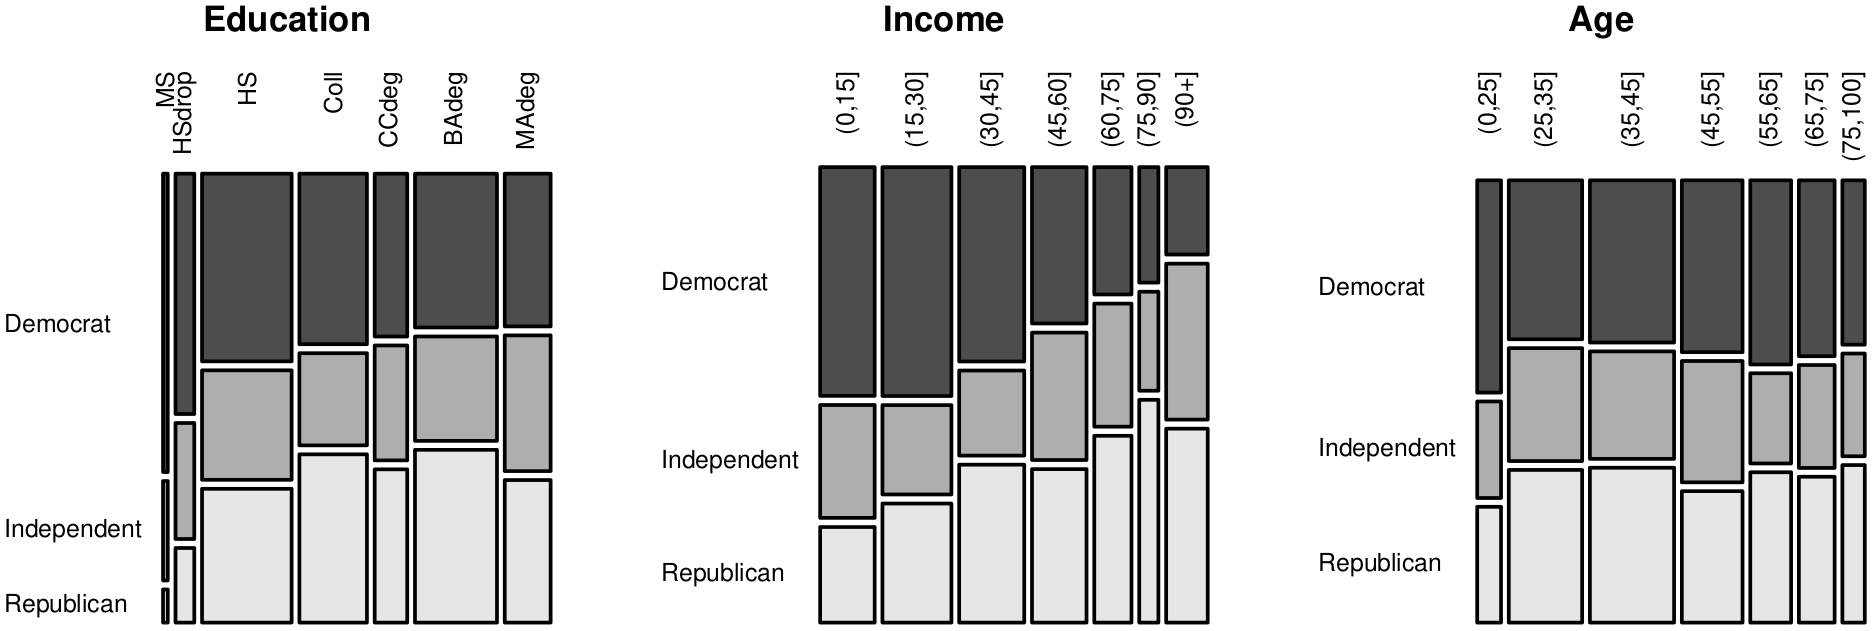
\includegraphics[width=0.7\textwidth]{sections/GLM/images/mosaic}

\subsubsection{Mulinominal Logit Model}
Let $Y_\ell$ be a random variable coding the response categories with values
$1,2,\ldots,L$.
Then $\pi_{i\ell} = P(Y_i = \ell)$ is the probability that the response of the
$i^\text{th}$ observation falls into the $\ell^\text{th}$ category.
Let $y_{i\ell}$ be the number of observations falling into category $\ell$.
We define
\begin{align*}
n_i
:=
\sum_{\ell=1}^L y_{i\ell},
\end{align*}
which is the number of individual in observation $i$.
The vector $[y_{i1},\ldots,y_{iL}]^T$ conditioned on the total $n_i$ follows a
\textbf{multinomial distribution}
\begin{align*}
P\left(
Y_{i1} = y_{i1}, Y_{i2} = y_{i2}, \ldots, Y_{iL} = y_{iL}
\middle\vert
\sum_{\ell=1}^L y_{i\ell} = n_i
\right)
=
n!\prod_{\ell=1}^L \frac{\pi_{i1}^{y_{i1}}}{y_{i\ell}}
\end{align*}
We apply a similar idea as with the logit model
\begin{align*}
\log\frac{P\left(Y_{i\ell} = y_{i\ell} \middle\vert x_i\right)}
{P\left(Y_{i1} = y_{i1} \middle\vert x_i\right)}
\log \frac{\pi_{i\ell}}{\pi_{i1}}
=
\eta_{i\ell}
=
\beta_{0\ell} + \beta_{1\ell} x_i^{(1)} + \ldots + \beta_{m\ell} x_i^{(m)}
\quad
\forall \ell = 2,3,\ldots,L
\end{align*}

\subsubsection{Oridnal Multinomial Response}
Suppose we have $L$ ordered categories and
for and individual $i$ with ordinal response $Y_i$,
where $Y_i$ is coded as $1,2,\ldots,L$.
With an ordered response,
it is often easier and more powerful to work with cumulative probabilities
$\gamma_{i\ell} = P(Y_i \leq \ell)$.
These probabilities are obviously increasing.
$\gamma_{i\ell}=1$, so we need only to model $(L-1)$ probabilites.
We consider model approaches that have the form
\begin{align*}
g(\gamma_{i\ell})
=
\alpha_l - x_i^T \beta
\quad
\forall \ell=1,\ldots,L-1
\end{align*}
The latent variable may be thought of as the underlying continuous but
unobserved response.
In practice, we are limited to observing $Y_i$ which are discretized version of
$T_i$ with
\begin{align*}
Y_i = \ell,
\text{ if }
\widetilde{\alpha}_{\ell-1} < T_i \leq \alpha_\ell
\end{align*}
The thresholds $\widetilde\alpha_\ell$ do not need to be equidistant and
they are usually not known a priori,
but estimated from the data.

\subsubsection{Inference}
For inferring whether the $k^\text{th}$ explanatory variable
has a significant impact on the response,
we cannot perform individual hypothesis tests anymore.
Thus, we have to resort to a comparison of nested models,
which will as before be based on deviance differences.